% MIWAI 2026, paper 122. One-page graphical abstract, second layout.
%
% v1 grew by accretion: each new block went into whatever space was left, so
% the method band ended up carrying four things and the evidence band three,
% on a grid drawn for three and two. The Grad-CAM pair sat in a gap under the
% frozen branch, four elements in the top band had four different vertical
% anchors, and the lower band stopped 34mm short of the right margin.
%
% This is three blocks per band, both bands running the full measure, one
% gutter width, and a shared top and bottom rail in each band.
%
% This is a rebuild, not a revision. The previous version was three equal
% rounded cards labelled THE PROBLEM / THE MODEL / THE RESULT. That skeleton is
% the clinical "visual abstract" invented at Annals of Surgery in 2016 for
% tweeting trial results: population, intervention, outcome. It belongs to
% clinical-trial journals talking to a lay audience. This is an AI methods
% paper at an LNAI venue, where the real convention is the CVPR-style teaser
% and the Elsevier single-canvas graphical abstract: one continuous surface,
% no card frames, no chrome, the mechanism drawn rather than asserted.
%
% So: one canvas. The scan anchors it, the pipeline is drawn as a pipeline, and
% the headline sits on an axis next to the baseline it beats, because a number
% on an axis demonstrates and a number in a coloured box only asserts.
%
% Colour is the one deliberate constraint. Radiology is greyscale, so the page
% is greyscale, and the single accent is reserved entirely for the Severe class
% and its recall. Nothing else on the page is coloured. The two branches are
% told apart by solid against dashed, which encodes the actual difference
% (trained against frozen) instead of decorating it.
%
% Type is Charter, a printed-text serif, with Avenir Next Condensed only for
% annotation on and around the image, the way a viewer overlays a scan.
%
% Build (needs lualatex for system fonts):
%   lualatex -interaction=nonstopmode infographic.tex
%   pdftoppm -png -scale-to-x 1920 -scale-to-y 1080 infographic.pdf infographic
\documentclass[12pt]{article}
\usepackage[paperwidth=320mm,paperheight=180mm,margin=0mm]{geometry}
\usepackage{fontspec}
\setmainfont{Charter}
\newfontfamily\cond{Avenir Next Condensed}
\usepackage{graphicx}
\usepackage{tikz}
\usetikzlibrary{arrows.meta,positioning,calc,decorations.pathreplacing}
\pagestyle{empty}
\setlength{\parindent}{0pt}

% The first palette used warm, olive-tinted neutrals (F7F7F5, DFDFDA, B8B8B2)
% with a brick accent. Tinted neutrals read as dirty rather than as restrained,
% and the whole page came out dusty. These are clean, faintly cool greys, which
% is what reads as clinical, and the accent now has real chroma.
\definecolor{paper}{HTML}{F8F9FA}
\definecolor{ink}{HTML}{000000}
\definecolor{ink70}{HTML}{55595E}
\definecolor{rule}{HTML}{C9CDD2}
\definecolor{track}{HTML}{E3E7EB}
\definecolor{track2}{HTML}{9AA3AC}
% Matches the Severe red of the paper's own class-distribution figure, so the
% two artefacts agree. Used for the Severe class and its recall, nothing else.
\definecolor{signal}{HTML}{E23B3B}
\definecolor{slot}{HTML}{E3E7EB}
% A second accent, earning its place: it marks everything that is actually
% trained. Blue path against grey dashed frozen blocks is the paper's headline
% about parameter efficiency, drawn instead of stated.
\definecolor{trained}{HTML}{1971C2}
\definecolor{trainedbg}{HTML}{EDF4FC}
\definecolor{bar2}{HTML}{6E7781}
\definecolor{waffle}{HTML}{C3C9CF}
\definecolor{grid}{HTML}{DDE2E6}

\newcommand{\arr}{\raisebox{0.18ex}{\tikz[baseline=-0.55ex]
  \draw[-{Stealth[length=1.9mm,width=1.6mm]},line width=0.5mm](0,0)--(4.4mm,0);}}

\begin{document}
\begin{tikzpicture}[x=1mm,y=1mm,
  box/.style={draw=trained, line width=0.45mm, fill=trainedbg, minimum height=18mm,
              align=center, inner sep=2mm, font=\fontsize{11}{13}\selectfont},
  frz/.style={draw=ink70, line width=0.4mm, dash pattern=on 1.4mm off 1.1mm,
              fill=white, minimum height=18mm, align=center, inner sep=2mm,
              font=\fontsize{11}{13}\selectfont},
  flow/.style={-{Stealth[length=2.2mm,width=1.8mm]}, line width=0.35mm, ink},
  tflow/.style={-{Stealth[length=2.2mm,width=1.8mm]}, line width=0.45mm, trained}]

\fill[paper] (0,0) rectangle (320,180);

%% ------------------------------------------------------------- title
\node[anchor=base west, font=\fontsize{24}{27}\selectfont]
     at (16,164) {A Two-Branch Hybrid Model for Lumbar Disc Grading};
\node[anchor=base west, text=ink70, font=\fontsize{10}{12}\selectfont]
     at (16,155) {Ha Trung Kien and Phan Trong Nhan, Ho Chi Minh City University of Technology, Vietnam};
\node[anchor=base east, text=ink70, font=\fontsize{10}{12}\selectfont]
     at (304,155) {MIWAI 2026, paper 122};
\draw[rule, line width=0.2mm] (16,150) -- (304,150);

%% ============================================ METHOD BAND, y 86 to 146
% Three blocks: scan 30, pipeline 136, prompts 100, gutters 10.
\node[anchor=south west, inner sep=0] at (16,90)
     {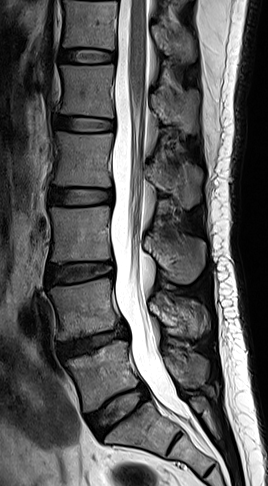
\includegraphics[width=30mm,height=54mm]{mri_sagittal_panel.png}};
\node[anchor=base west, text=ink70, font=\cond\fontsize{9}{11}\selectfont]
     at (16,86) {Sagittal T2, 5 IVD levels};

\node[box, minimum width=50mm] (bxA) at (97,128) {3D ResNet-34 + CBAM\\[2pt]
     {\cond\fontsize{9}{11}\selectfont trainable}};
\node[frz, minimum width=50mm] (bxB) at (97,100) {BiomedCLIP encoder\\[2pt]
     {\cond\fontsize{9}{11}\selectfont frozen}};
\node[box, minimum width=48mm, minimum height=13mm] (fus) at (167,114) {concat MLP};

\draw[ink, line width=0.35mm] (48,114) -- (58,114);
\draw[ink, line width=0.35mm] (58,128) -- (58,100);
\draw[tflow] (58,128) -- (bxA.west);
\draw[flow]  (58,100) -- (bxB.west);
\draw[trained, line width=0.45mm] (bxA.east) -- (132,128);
\draw[ink70, line width=0.35mm] (bxB.east) -- (132,100);
\draw[trained, line width=0.45mm] (132,128) -- (132,114);
\draw[ink70, line width=0.35mm] (132,114) -- (132,100);
\draw[tflow] (132,114) -- (fus.west);
\draw[tflow] (fus.east) -- (200,114);
\node[anchor=south, text=ink70, font=\cond\fontsize{9}{11}\selectfont]
     at (196,115.5) {cosine sim.};

%% prompts, centred on the pipeline
\node[anchor=base west, font=\fontsize{13}{16}\selectfont]
     at (204,140) {No classifier head, just text prompts.};
\node[anchor=base west, text=ink70, font=\fontsize{10}{13}\selectfont] at (208,130) {normal or mild};
\node[anchor=base west, text=ink70, font=\fontsize{10}{13}\selectfont] at (208,124) {moderate};
\node[anchor=base west, text=signal, font=\fontsize{10}{13}\selectfont] at (208,118) {severe};
\draw[ink70, line width=0.25mm, decorate,
      decoration={brace, amplitude=1.6mm, mirror}] (237,116.5) -- (237,132);
\node[anchor=base west, text=ink70, font=\fontsize{10}{13}\selectfont] at (241,123.5)
     {spinal canal stenosis};
\node[anchor=base west, text=ink70, font=\cond\fontsize{9}{11}\selectfont] at (208,109)
     {three grades per condition; the image is the only per-case input};
\node[anchor=base west, text=trained, font=\cond\fontsize{9}{11}\selectfont]
     at (204,100) {edit the phrases, get a new label space, no gradient updates};
\node[anchor=base west, text=ink70, font=\cond\fontsize{9}{11}\selectfont]
     at (204,92) {Zero-shot macro F1, SPIDER labels unseen in training};
\node[anchor=base west, font=\fontsize{9.5}{12}\selectfont] at (208,86) {disc bulging \ 0.613};
\node[anchor=base west, text=ink70, font=\fontsize{9.5}{12}\selectfont] at (256,86) {spondylolisthesis \ 0.028};

\draw[rule, line width=0.2mm] (16,80) -- (304,80);

%% ============================================ EVIDENCE BAND, y 30 to 76
% Three blocks: distribution 84, Grad-CAM 76, results 108, gutters 10.
\node[anchor=base west, text=ink70, font=\cond\fontsize{9}{11}\selectfont]
     at (16,72) {Severity distribution, RSNA 2024};
\node[anchor=south west, inner sep=0] at (16,32)
     {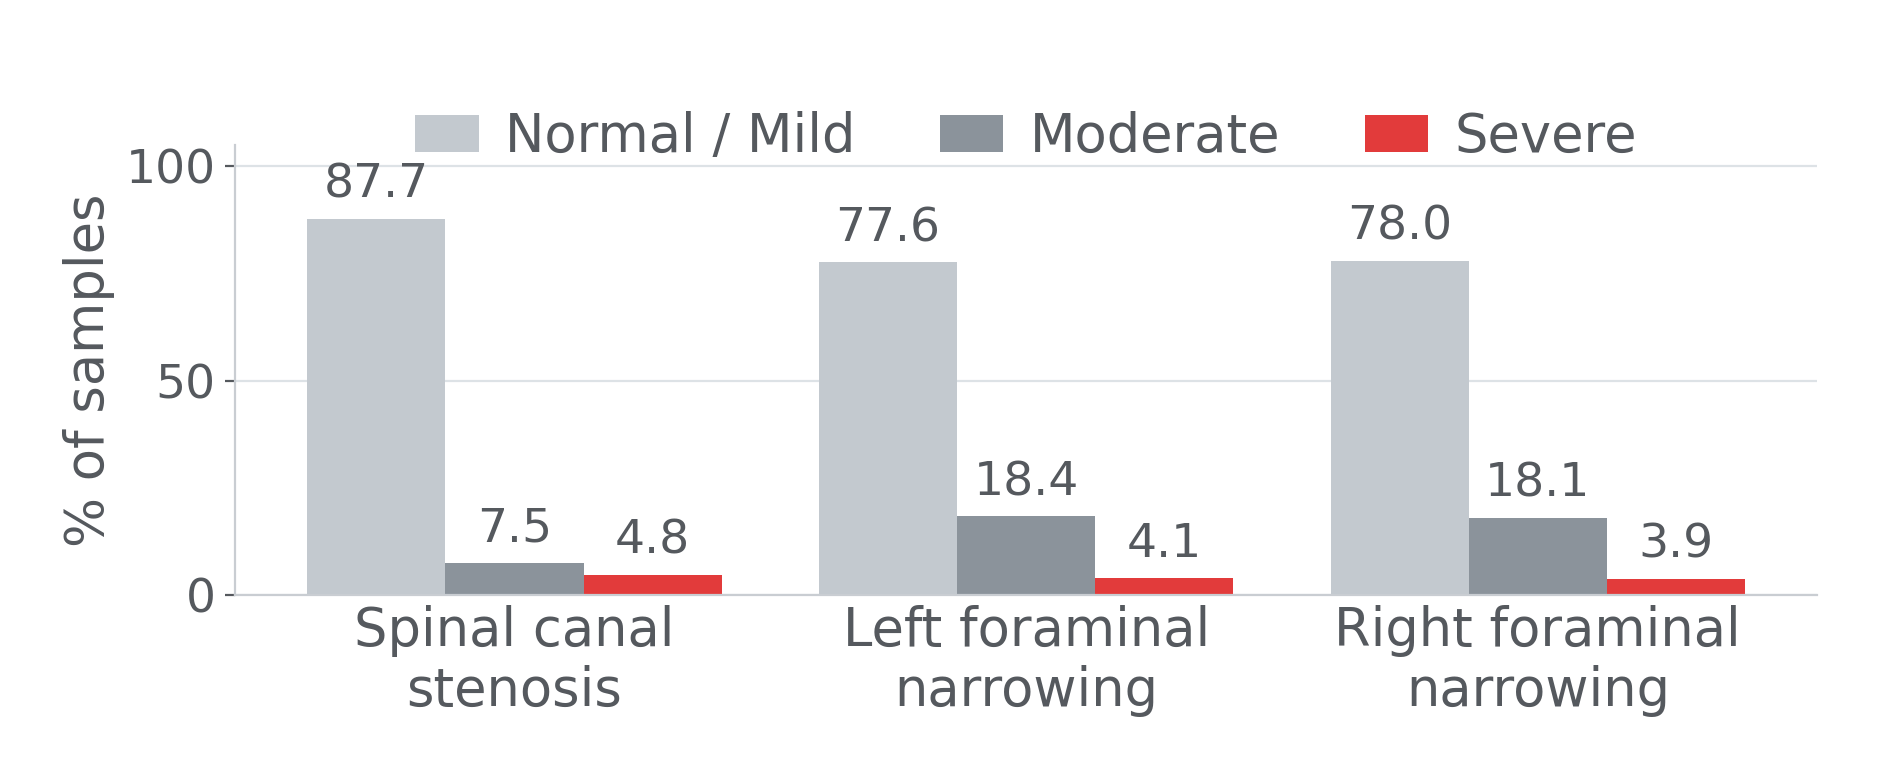
\includegraphics[width=84mm]{rsna_dist_compact.png}};

\draw[rule, line width=0.2mm] (105,32) -- (105,72);

\node[anchor=base west, text=ink70, font=\cond\fontsize{9}{11}\selectfont]
     at (110,72) {Grad-CAM, a Severe spinal canal case};
\node[anchor=south west, inner sep=0] at (110,46)
     {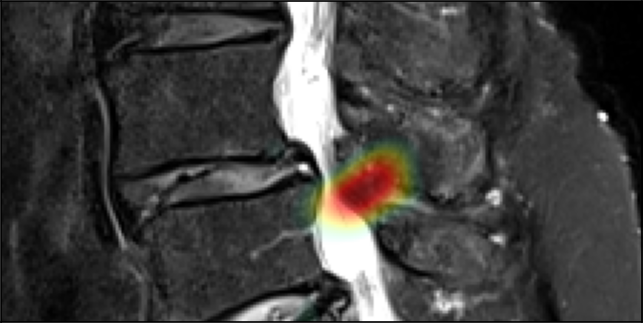
\includegraphics[width=36mm]{gradcam_nocbam.png}};
\node[anchor=south west, inner sep=0] at (150,46)
     {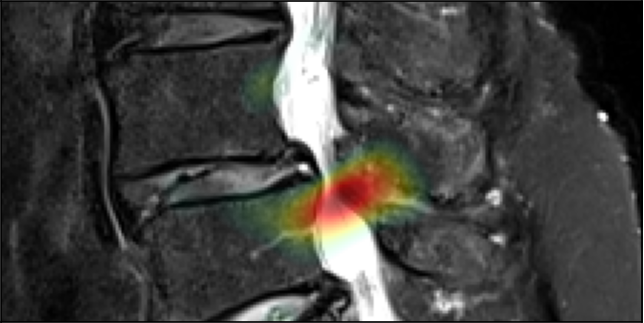
\includegraphics[width=36mm]{gradcam_cbam.png}};
\node[anchor=base west, text=ink70, font=\cond\fontsize{9}{11}\selectfont] at (110,41) {without CBAM};
\node[anchor=base west, text=ink70, font=\cond\fontsize{9}{11}\selectfont] at (150,41) {with CBAM};

\draw[rule, line width=0.2mm] (191,32) -- (191,72);

\node[anchor=base west, text=ink70, font=\cond\fontsize{9}{11}\selectfont]
     at (196,72) {Severe-class recall, RSNA 2024 validation, 3 seeds};
\foreach \x in {243.5,261,278.5,296} \draw[grid, line width=0.2mm] (\x,44) -- (\x,67);
\draw[rule, line width=0.3mm] (226,44) -- (226,67);
\fill[bar2]   (226,58) rectangle ++(8.6,6);
\fill[signal] (226,48) rectangle ++(34.0,6);
\node[anchor=base east, text=ink70, font=\cond\fontsize{9}{11}\selectfont] at (222,60) {SpineNetV2};
\node[anchor=base east, text=signal, font=\cond\fontsize{9}{11}\selectfont] at (222,50) {hybrid (ours)};
\node[anchor=base west, text=ink70, font=\fontsize{10}{12}\selectfont] at (238,60) {12.3\%};
\node[anchor=base west, text=signal, font=\fontsize{14}{16}\selectfont] at (264,49.5) {48.6\%};
\foreach \x/\lab in {226/0,243.5/25,261/50,278.5/75,296/100} {
  \node[anchor=base, text=ink70, font=\cond\fontsize{8.5}{10}\selectfont] at (\x,40) {\lab};}
\node[anchor=base west, text=ink70, font=\cond\fontsize{8.5}{10}\selectfont] at (298.5,40) {\%};
\node[anchor=base west, text=ink70, font=\cond\fontsize{9}{11}\selectfont] at (196,33)
     {Severe F1 0.152 to 0.356\quad Severe AUC 0.872 to 0.899};

%% ------------------------------------------------------------- provenance
\node[anchor=base west, text=ink70, font=\fontsize{8.5}{11}\selectfont]
     at (16,21) {Severity distribution and Grad-CAM are both from the paper; the saliency map is qualitative support, not by itself proof of a mechanism.};
\node[anchor=base west, text=ink70, font=\fontsize{8.5}{11}\selectfont]
     at (16,15) {SpineNetV2 is its grading backbone retrained here, not the published pipeline. Zero-shot: one RSNA-trained model, frozen, on the full SPIDER cohort (1{,}439 IVDs).};

\end{tikzpicture}
\end{document}
